\documentclass[../TDE8_filtrage.tex]{subfiles}%

\begin{document}
\section[s]"1"{Filtrage et spectres}

\enonce{%
	Un signal périodique $e(t)$ (de fréquence \SI{1}{kHz}), dont le spectre est
	donné en figure 1, est envoyé à l'entrée de trois filtres différents. On
	effectue l'analyse spectrale du signal de sortie pour chaque filtre, les
	spectres obtenus sont donnés en figure 2, 3 et 4.

	\begin{center}
		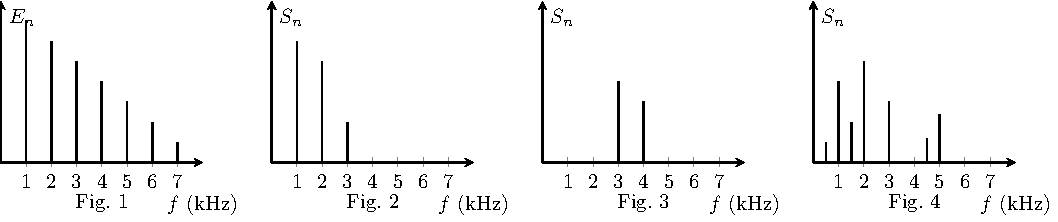
\includegraphics[width=\linewidth]{spectres_plain}
	\end{center}
}

\QR{%
	Quelles caractéristiques de chaque filtre peut-on déduire de ces spectres~?
}{%
	\ifprof{%
		\vspace{-15pt}
	}%
	\begin{enumerate}
		\item Sur la figure deux, les basses fréquences sont globalement conservées,
		      et les fréquences à partir de \SI{3}{kHz} sont fortement atténuées voire
		      coupées~: \textbf{c'est un passe-bas}.
		\item Sur la figure trois, seules les fréquences entre 3 et \SI{4}{kHz} sont
		      gardées, les fréquences supérieures ou inférieures sont coupées~:
		      \textbf{c'est un passe-bande}.
		\item Sur la figure quatre, on ne distingue pas de relation simple vue en
		      cours~; on remarque de plus que de nouvelles fréquences apparaissent, ce
		      qui n'est pas le cas dans le filtrage linéaire~: c'est un \textbf{filtre
			      non-linéaire}.
	\end{enumerate}
}

\end{document}
